\documentclass{article}
\usepackage{amsmath}
\usepackage{mathtools}
\usepackage{gensymb}
\usepackage[a4paper,inner=1.5cm,outer=1.5cm,top=2cm,bottom=0.5cm]{geometry} 
\usepackage{xcolor}                    
\usepackage{tikz}                           
\usepackage{multicol}
\usepackage{pgfplots}
\usetikzlibrary{calc}
\usetikzlibrary{intersections}
\usetikzlibrary{intersections,calc,angles,quotes}
\usetikzlibrary{shapes,arrows,positioning,decorations.pathreplacing,calc}
\usetikzlibrary{calc,angles,positioning,intersections,quotes,decorations.markings}
\usepackage{tkz-euclide}
\usetikzlibrary{backgrounds}
\usetikzlibrary{calc,through}
\usetikzlibrary{angles}
\usetikzlibrary{fadings}
\usetikzlibrary{shapes.geometric}
\usetikzlibrary{shapes.symbols}
\usepackage{draftwatermark}
\usepackage{mathptmx}

\SetWatermarkText{\textcolor{black!30}{Mathema Shukur}}
\SetWatermarkFontSize{2 cm}
\usepackage[utf8]{inputenc}
\usepackage{fontspec}

\setmainfont{[Kalpurush.ttf]}
\newfontface{\en}{[Arial.ttf]} %%this is optional, if you want to use a secondary font. Any english font is supported
\newlength\Radius
\setlength\Radius{4cm}
\begin{document} 
	\Large
	\textcolor{red}{Welcome To} 
	\\
	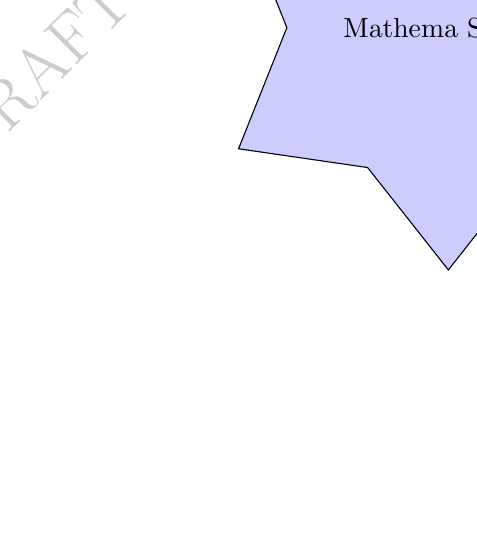
\begin{tikzpicture}
		\tikz \node [fill=blue!20,star,star points=6,draw] {Mathema Shukur };
	\end{tikzpicture}
	\\
	যাদের জন্যে প্রযোজ্যঃ  	\textcolor{magenta}{একাদশ ও দ্বাদশ শ্রেণীর শিক্ষার্থী} \\
	বিষয়ঃ \textcolor{magenta}{উচ্চতর গণিত ১ম পত্র} \\
	অধ্যায়ঃ \textcolor{magenta}{৩-সরলরেখা}\\ 
	Subtopicঃ  \textcolor{magenta}{ অক্ষরেখার সমীকরণ নির্ণয় করা equation of axes }\\
	\\
Co-ordinate geometry is a marriage of pure geometry and algebra\\
\\
 The core concept is that on a 2-dimensional (Euclidean) plane, any point can be represented by a pair of real numbers, using two non-parallel straight lines. \\
 \\
 The point where these two non-parallel reference lines meet is termed the origin of the reference axis.\\
 \\
  By convention, one axis is called the x-axis and one the y-axis.\\
\\
যে সরলরেখার প্রতিটি বিন্দুর কোটি  শূন্য তাকে $x-$ অক্ষ বলে \\
\\
 $x-$ অক্ষের সমীকরণ $y=0$\\
 \\
 যে সরলরেখার প্রতিটি বিন্দুর ভূজ  শূন্য তাকে $y-$ অক্ষ বলে \\
 \\
 $y-$ অক্ষের সমীকরণ $x=0$\\
 \\
 $x$ অক্ষ এবং  $y$ অক্ষ পরস্পরকে লম্বভাবে ছেদ করে । ছেদ বিন্দুকে মূলবিন্দু বলে $(0,0)$ \\
 \\ 
 \begin{tikzpicture}[transform shape,scale=1]
 	\draw [-latex,thick,blue](-6,0) -- (6,0) node[right] {$x$} coordinate(x axis);
 	\draw [-latex,thick,red](0,-6) -- (0,6) node[above] {$y$} coordinate(y axis);
 	\fill[black] (0,0) circle (1 mm);
 	\node at (0.8,-0.3) {$\textcolor{purple}{O(0,0)}$};	
 	\node at (1.5,0.4) {$\textcolor{cyan}{90\degree}$};	
 	\node at (3,0.5) {$\textcolor{magenta}{(3,0) }$};	
 			\fill[blue] (3,0) circle (1 mm);
 			\node at (3,0.5) {$\textcolor{blue}{(3,0) }$};	
 				\fill[blue] (5,0) circle (1 mm);
 			\node at (5,0.5) {$\textcolor{blue}{(5,0) }$};	
 			\fill[blue] (-2,0) circle (1 mm);	
 			\node at (-2,0.5) {$\textcolor{blue}{(-2,0) }$};	
 				\fill[blue] (-4,0) circle (1 mm);	
 			\node at (-4,0.5) {$\textcolor{blue}{(-4,0) }$};	
 		\fill[red] (0,2) circle (1 mm);	
 	\node at (0.7,2) {$\textcolor{red}{(0,2) }$};	
 		\fill[red] (0,5) circle (1 mm);	
 	\node at (0.7,5) {$\textcolor{red}{(0,5) }$};	
 		\fill[red] (0,-3) circle (1 mm);	
 	\node at (1,-3) {$\textcolor{red}{(0,-3) }$};			
 	\draw[color=cyan,ultra thick, ->] (1,0) arc (0:90:1cm);
 \end{tikzpicture}
 \\
(1) $x$ অক্ষের উপর লম্ব এবং মূল বিন্দুগামী রেখার সমীকরণ নির্ণয় কর\\
\\ 
\begin{tikzpicture}[transform shape,scale=1]
	\draw [-latex,thick,blue](-6,0) -- (6,0) node[right] {$x$} coordinate(x axis);
	\draw [-latex,thick,red](0,-6) -- (0,6) node[above] {$y$} coordinate(y axis);
	\fill[black] (0,0) circle (1 mm);
	\node at (0.3,-0.3) {$\textcolor{purple}{O}$};	
	\node at (1.5,0.4) {$\textcolor{cyan}{90\degree}$};	
	\draw[color=cyan,ultra thick, ->] (1,0) arc (0:90:1cm);
		\node at (1,3) {$\textcolor{red}{x=0}$};	
\end{tikzpicture}\\
(2) $y$ অক্ষ থেকে $4$ একক দূরত্বে $x$ অক্ষের উপর অবস্থিত বিন্দুর স্থানাঙ্ক নির্ণয় কর \\
 \begin{tikzpicture}[transform shape,scale=1]
	\draw [-latex,thick,blue](-6,0) -- (6,0) node[right] {$x$} coordinate(x axis);
	\draw [-latex,thick,red](0,-6) -- (0,6) node[above] {$y$} coordinate(y axis);
	\fill[black] (0,0) circle (1 mm);
	\node at (-0.3,-0.3) {$\textcolor{purple}{O}$};	
	\fill[blue] (4,0) circle (1 mm);
	\node at (4,0.5) {$\textcolor{blue}{(4,0) }$};	
		\draw [cyan,very thick,decorate,decoration={brace,amplitude=12pt,mirror,raise=3ex}]
	(0,0) -- (4,0);
		\node at (2,-1.5) {$\textcolor{cyan}{4 }$};	
\end{tikzpicture}\\
(3) $x$ অক্ষ থেকে $-3$ একক দূরত্বে $y$ অক্ষের উপর অবস্থিত বিন্দুর স্থানাঙ্ক নির্ণয় কর \\
\begin{tikzpicture}[transform shape,scale=1]
	\draw [-latex,thick,blue](-6,0) -- (6,0) node[right] {$x$} coordinate(x axis);
	\draw [-latex,thick,red](0,-6) -- (0,6) node[above] {$y$} coordinate(y axis);
	\fill[black] (0,0) circle (1 mm);
	\node at (0.3,-0.3) {$\textcolor{purple}{O}$};	
	\fill[red] (0,-3) circle (1 mm);
	\node at (1,-3) {$\textcolor{red}{(0,-3) }$};	
	\draw [cyan,very thick,decorate,decoration={brace,amplitude=12pt,mirror,raise=3ex}]
	(0,0) -- (0,-3);
	\node at (-1.5,-1.5) {$\textcolor{cyan}{-3 }$};	
\end{tikzpicture}
\\
(5) $a$ এর মান কত হলে  $(a+1,a-4)$ বিন্দুটি $x-$ অক্ষের উপর  অবস্থিত হবে \\
\\ 
$x-$ অক্ষের উপর  অবস্থিত প্রতিটি বিন্দুর কোটি শূন্য \\
\\
$a-4=0,\qquad  a=4$\\
\\
\vspace{6cm}
\\
$x$ অক্ষের সমান্তরাল  রেখায় প্রতিটি বিন্দুর কোটি একটি স্থির সংখ্যা $(b)$ \\
\\
 $x$ অক্ষের সমান্তরাল  রেখার সমীকরণ $y=b$\\
 \\ 
(6) $(-3,4)$ বিন্দুগামী এবং  $x$ অক্ষের সমান্তরাল রেখার সমীকরণ নির্ণয় কর\\
\\ 
\begin{tikzpicture}[transform shape,scale=1]
	\draw [-latex,thick](-6,0) -- (6,0) node[right] {$x$} coordinate(x axis);
	\draw [-latex,thick](0,-6) -- (0,6) node[above] {$y$} coordinate(y axis);
	\fill[black] (0,0) circle (1 mm);
		\fill[magenta] (-3,4) circle (1 mm);
	\node at (-0.3,-0.3) {$\textcolor{purple}{O}$};	
	\node at (-3,0004.5) {$\textcolor{magenta}{(-3,4) }$};	
	\node at (4.5,3.5) {$\textcolor{magenta}{y=4}$};
		\draw[very thick,magenta] (5,4)--(-4,4);
\end{tikzpicture}
\\
$y$ অক্ষের সমান্তরাল  রেখায় প্রতিটি বিন্দুর ভুজ একটি স্থির সংখ্যা $(a)$  \\
\\
$y$ অক্ষের সমান্তরাল  রেখার সমীকরণ $x=a$\\
\\ 
(7) $(3,-2)$ বিন্দুগামী এবং $y$ অক্ষের সমান্তরাল রেখার সমীকরণ নির্ণয় কর\\
\\ 
\begin{tikzpicture}[transform shape,scale=1]
	\draw [-latex,thick](-6,0) -- (6,0) node[right] {$x$} coordinate(x axis);
	\draw [-latex,thick](0,-6) -- (0,6) node[above] {$y$} coordinate(y axis);
	\fill[black] (0,0) circle (1 mm);
	\fill[magenta] (3,-2) circle (1 mm);
	\node at (-0.3,-0.3) {$\textcolor{purple}{O}$};	
	\node at (4,-2) {$\textcolor{magenta}{(3,-2) }$};	
	\node at (4,2) {$\textcolor{magenta}{x=3}$};
	\draw[very thick,magenta] (3,4)--(3,-4);
\end{tikzpicture}
\end{document}